El filtro Decode, obtiene un mensaje a partir de los bytes de la entrada, proces\'andolos primero y luego qued\'andose con los bits relevantes para la 
decodificaci\'on.

\subsubsection{Implementación en C}
En un ciclo principal, se recorren los bytes de la fuente, hasta terminar de recorrer la imagen o alcanzar el tamaño recibido por par\'ametro. Dentro de 
este ciclo hay otro, que recorre de a 4 bytes. Los obtiene primero el c\'odigo de la operación a aplicar, luego los bits que ser\'an procesados y luego 
se realiza el algoritmo correspondiente. En cada iteraci\'on del ciclo interior, en una variable que contiene el byte decodificado, inserta los bits 
procesados en la posici\'on que les corresponde. Al terminar con el cuarto byte, pega ese valor en la salida y avanza los punteros y variables para 
continuar con el siguiente grupo de bytes.

\subsubsection{Implementación en Assembler}
El ciclo del algoritmo obtiene en primer lugar 16 bytes de la fuente. Luego, con una m\'ascara obtengo los bits 2 y 3 de cada byte en un registro. Luego 
con otras m\'ascaras, se obtienen los bytes a los que se les debe sumar 1 en un registro y a los que se debe restar 1 en otro. El pr\'oximo paso, niega 
los bits de los bytes cuyo c\'odigo de opraci\'on es 3. A ese resultado, se le suma 1 al registro usando la m\'ascara obtenida anteriormente, y lo mismo 
se hace para restar 1 usando la otra m\'ascara. Despu\'es de eso, se borran todos los bits que no interesan, dejando solo los bits 0 y 1 de cada byte.\newline
Para juntarlos y armar los bytes decodificados, en diferentes registros, se dejan solo los pares de bits que van en las posiciones 0 y 1, 2 y 3, 4 y 5 , 
6 y 7. Luego, con pshufb y las m\'ascaras correspondientes, llevo esos bits manteniendo sus posiciones, pero a los primeros 3 bytes del registro. Y 
finalmente con la instrucci\'on POR se guardan en un solo registro todos los bits en su posici\'on correspondiente. Finalmente se guarda ese registro en 
la posición del output. Como solo los primeros 3 bytes eran reelevantes para el output, el puntero se avanza solo 3 lugares. En la fuente en cambio, 
aumento 12 lugares la posici\'on. Esto se hace as\'i porque cada pixel ocupa 3 bytes, y para formar un byte de la salida se necesitan 4 bytes. Avanzar de
 a 12 la fuente y de a 3 el destino entonces, es conveniente para avanzar de forma m\'as ordenada y segura.

\subsubsection{Resultados}
La diferencia principal entre el c\'odigo escrito en lenguaje C y el c\'odigo ASM, es la cantidad de accesos a memoria realizados en cada iteraci\'on. Otra diferencia puede verse en la cantidad de bytes que puden ser procesados simultaneamente durante el mismo ciclo. Mientras que en C leemos y procesamos un byte por vez, el c\'odigo ASM nos permite acceder y procesar 16 bytes en simultaneos. De todas maneras, en este caso trabajamos con 12 bytes que es un numero mas \'util ya que es m\'ultiplo de 3 (cantidad de bytes pos pixel)  y de 4 (cantidad de bytes por cada caracter).
\newline
Pudiendo levantar de a 16 bytes en memoria, podr\'ia esperarse que el c\'odigo asm demorase una diesiseiava parte de la cantidad de ciclos que demora el c\'odigo en C. Pero debemos tener en cuenta que en nuestro caso estamos aprovechando solo 12 de los 16 bytes que leemos en cada iteraci\'on por lo tanto es más acertado evaluar como si solo leyeramos 12 bytes. Adem\'as, hay que tener en cuenta que las instrucciones SSE pueden necesitar más ciclos que las operaciones comunes que usamos en el C, eso disminuye un poco la performance en la comparación. Viendo el promedio de ciclos necesitados por cada c\'odigo en promedio, estamos en la mayor\'ia de los casos en cifras cercanas a 10.35, por lo tanto, concluimos que para la mayoría de los casos, esa es la relaci\'on de performance entre los códigos.
\newline

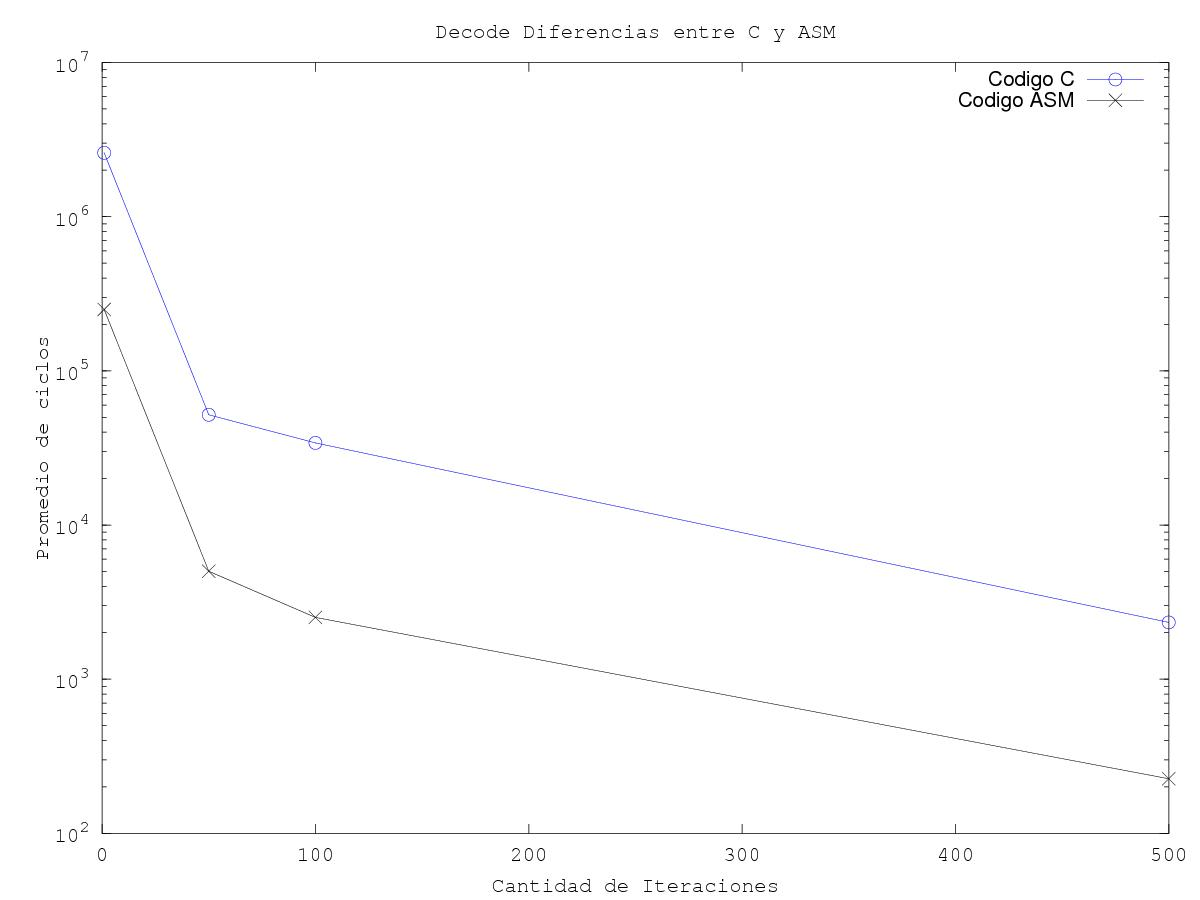
\includegraphics[scale=0.7]{imagenes/octave1.jpg}

Probando con im\'agenes de distintos tamaños, una de 1920 X 1080 p\'ixeles y otra de 640 x 480 p\'ixeles, sucedi\'o en ambos casos que hubo un aumento en la diferencia entre los c\'odigos, pero se mantuvo, para las dos im\'agenes y, para distinta cantidad de iteraciones, un promedio de aproximadamente, por lo que no presentan grandes cambios con la imagen original. 

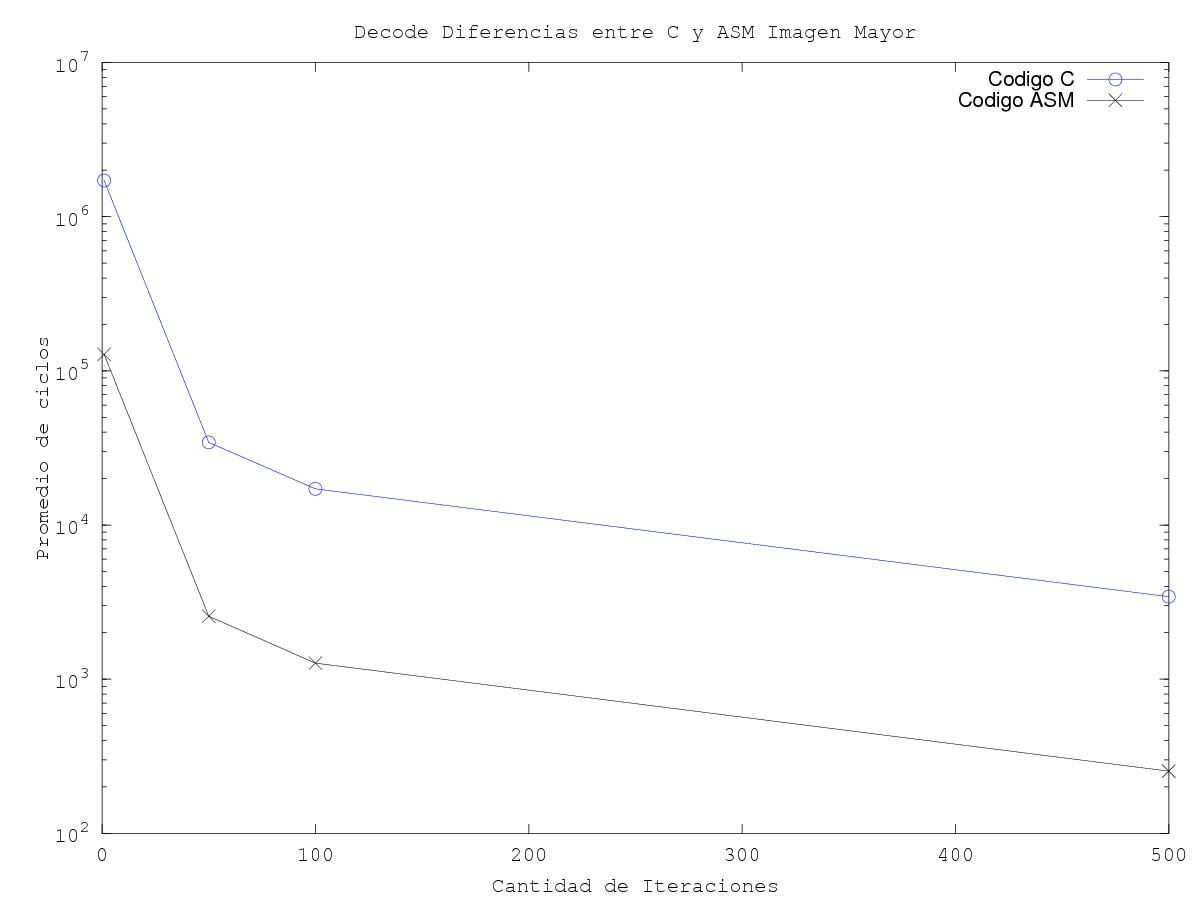
\includegraphics[scale=0.7]{imagenes/DecodeMayor.jpg}

